
%(BEGIN_QUESTION)
% Copyright 2015, Tony R. Kuphaldt, released under the Creative Commons Attribution License (v 1.0)
% This means you may do almost anything with this work of mine, so long as you give me proper credit

\noindent
{\bf Demonstration Program -- contact and coil instructions} 

\vskip 10pt

An important technique for learning any programming language -- Ladder Diagram PLC programming included -- is to write simple ``demonstration'' programs showcasing and explaining how particular instructions and programming constructs are supposed to work.  Since you have access to your own personal PLC, you can explore the elements of your PLC's programming language like a scientist would explore new specimens: subject them to tests and record how they respond.  This is how you will be able to teach yourself new models of PLC when you are working in your career, when you won't have textbooks to follow or training to show you exactly what to do.

\vskip 10pt

Write such a ``demonstration'' program for your PLC's {\it contact and coil} instructions, where discrete inputs on your PLC control discrete outputs on your PLC.  An acceptable demonstration program must meet these three criteria:

\begin{itemize}
\item{} {\bf Simple} -- nothing ``extra'' included in the program to detract from the fundamental behavior of the instruction(s) being explored
\vskip 5pt
\item{} {\bf Complete} -- nothing missing from the program relevant to the fundamental behavior of the instruction(s) being explored.  {\it For a contact and coil demonstration program, this includes normally-open and normally-closed contact instructions, as well as regular and retentive coil instructions.}
\vskip 5pt
\item{} {\bf Clearly documented} -- every rung clearly commented in your own words, every variable named
\end{itemize}

{\it Your instructor will challenge you to use this demonstration program to illustrate what you have learned about PLC counter instructions.}



\vskip 20pt \vbox{\hrule \hbox{\strut \vrule{} {\bf Suggested questions your demonstration program should answer:} \vrule} \hrule}

\begin{itemize}
\item{} Identify the different contact instruction types offered on your PLC.  Describe how each of them functions.
\item{} Identify the different coil instruction types offered on your PLC.  Describe how each of them functions.
\item{} What happens when two contact instructions are linked to the same bit address in the PLC's memory?  Do these contact instructions operated differently, or identically?
\item{} What happens when two coil instructions are linked to the same bit address in the PLC's memory, but driven to different states (e.g. one ``energized'' and the other ``de-energized'')?
\item{} Does your PLC offer a special type of contact or other bit-level instruction to detect the {\it transistion} of a bit from one state to another?  If so, how is this instruction used?
\item{} Where in the PLC's memory are the single-bit registers (e.g. input registers, output registers, and internal bit registers) located?  What symbol(s) are used to address each one?
\item{} Where in the PLC programming editor can you view the ``live'' status of contact and coil bits?
\item{} Experiment with using the {\it force} utility in your PLC to force certain bits to fixed values regardless of program operation.  How will the operation of your program be affected if a particular input bit is forced?  How will the operation of your program be affected if a particular output bit is forced?  How can you tell from the live program display that bits have been forced to fixed values?
\end{itemize}

\underbar{file i03354}
%(END_QUESTION)





%(BEGIN_ANSWER)

There are no answers provided here!  For help, consult the ``instruction set'' reference manual for your PLC, which will describe in detail how each type of instruction is supposed to function in your PLC.
 
%(END_ANSWER)





%(BEGIN_NOTES)

\noindent
{\bf Summary Quiz:}

The recommended summary quiz is to have \underbar{each student} demonstrate their PLCs running this demonstration program.  Demonstration programs should not be accepted unless and until they meet all three criteria listed in the question: they need to be {\it simple} (no extraneous features), {\it complete} (demonstrating {\it all} the necessary instructions), and {\it thoroughly documented} in the student's own words (every rung commented intelligently, every variable named).

\vskip 10pt

When checking students' demonstation programs, have them run the programs with their laptop PCs in online mode so they can view status highlighting and numerical values live, and {\it ask them to provide a running commentary of what they see the instructions doing.  If their commentary is lacking, challenge them to explore instruction behaviors that they have not yet done.}  Refer to the ``suggested questions'' for specific ideas on instruction behavior that may be explored in a demonstration program.

\vskip 10pt

This is by far the most important PLC program students will write today.  If there are other programs assigned in this day's plan, {\it prioritize this one}.  This point bears mentioning because a common error students make is to disregard the importance of a well-written demo program, instead tending to treat it as ``busywork'' and move on to ``more important'' assignments.  As the instructor your task is to explain why demonstration programs are important and to ensure students take them seriously:

\begin{itemize}
\item{} Demonstration programs are a powerful tool for self-instruction later when graduates will be challenged to learn some new PLC system.
\vskip 5pt
\item{} Demonstration programs may be re-run at a later date, which makes them ideal tools for review near the conclusion of the course.
\vskip 5pt
\item{} Demonstration programs require students to scientifically observe the PLC's programmed behavior, learning by {\it experiment} rather than learning by {\it direct instruction}.
\vskip 5pt
\item{} Well-written comments demand critical reflection on the part of the student, and also serve as practice for technical expression.
\end{itemize}








\vfil \eject

\noindent
{\bf Sample demonstration program for coil and contact instructions:} (for an Allen-Bradley MicroLogix PLC, showing only basic XIO, XIC, and OUT instructions; no retentive coils or special contacts shown)

$$\includegraphics[width=15.5cm]{i03354x01.eps}$$

%INDEX% PLC, demonstration program: contact and coil instructions

%(END_NOTES)


